% ============================================================
%  CS2311 Modern Operating System — Technical Report
%  Topic: KV Cache Memory Management in LLM Inference
%  Spring 2026 | Due: 17 May 2026
% ============================================================
\documentclass[10pt, a4paper]{article}

% ── Packages ────────────────────────────────────────────────
\usepackage[top=2.5cm, bottom=2.7cm, left=2.5cm, right=2.5cm]{geometry}
\usepackage{graphicx}
\usepackage{fancyhdr}
\setlength{\headheight}{1cm}
\usepackage{setspace}
\usepackage{titlesec}
\usepackage{hyperref}
\usepackage{cite}
\usepackage{caption}
\usepackage{subcaption}
\usepackage{booktabs}
\usepackage{amsmath, amssymb}
\usepackage{listings}
\usepackage{xcolor}
\usepackage{parskip}
\usepackage{microtype}

% ── Hyperref setup ──────────────────────────────────────────
\hypersetup{
    colorlinks = true,
    linkcolor  = black,
    citecolor  = blue!60!black,
    urlcolor   = blue!60!black,
}

% ── Code listing style ──────────────────────────────────────
\lstset{
    basicstyle   = \ttfamily\small,
    keywordstyle = \color{blue}\bfseries,
    commentstyle = \color{gray}\itshape,
    stringstyle  = \color{orange!80!black},
    numbers      = left,
    numberstyle  = \tiny\color{gray},
    frame        = single,
    breaklines   = true,
    captionpos   = b,
}

% ── Single spacing (as required) ────────────────────────────
\singlespacing

% ── Page style ──────────────────────────────────────────────
\pagestyle{fancy}
\fancyhf{}
% Replace "school_logo.png" with your actual logo filename.
% Put the image file in the same folder as this .tex file.
\fancyhead[R]{
\includegraphics[height=1.2cm]{school_logo.png}}
\fancyhead[L]{\small\textit{CS2311 Modern Operating System --- Technical Report}}
\fancyfoot[C]{\small\thepage}
\renewcommand{\headrulewidth}{0.4pt}
\renewcommand{\footrulewidth}{0pt}

\fancypagestyle{plain}{%
    \fancyhf{}
    \fancyhead[R]{
\includegraphics[height=1.2cm]{school_logo.png}}
    \fancyhead[L]{\small\textit{CS2311 Modern Operating System --- Technical Report}}
    \fancyfoot[C]{\small\thepage}
    \renewcommand{\headrulewidth}{0.4pt}
}

% ── Section formatting ──────────────────────────────────────
\titleformat{\section}{\large\bfseries}{\thesection}{1em}{}
\titleformat{\subsection}{\normalsize\bfseries}{\thesubsection}{1em}{}
\titleformat{\subsubsection}{\normalsize\itshape}{\thesubsubsection}{1em}{}

% ============================================================
\begin{document}

% ── Title Page ──────────────────────────────────────────────
\begin{titlepage}
    \centering
    \vspace*{1.5cm}

    
\includegraphics[width=0.25\textwidth]{school_logo.png}\\[1.5cm]

    {\LARGE\bfseries CS2311 Modern Operating System\\[0.4em]
    Technical Report}\\[1cm]

    \rule{\linewidth}{0.5pt}\\[0.5cm]
    {\huge\bfseries KV Cache Memory Management\\[0.3em]
    in LLM Inference:\\[0.3em]
    Challenges and Optimization Strategies}\\[0.3cm]
    \rule{\linewidth}{0.5pt}\\[2cm]

    \begin{minipage}[t][0.32\textheight][s]{\textwidth}
    \centering

        {\large
        \begin{tabular}{@{}rl@{}}
            \textbf{Student Name}  & Hengtao Wu \\[0.4em]
            \textbf{Student ID}    & 524031910038 \\[0.4em]
            \textbf{Course}        & CS2311 \\[0.4em]
            \textbf{Instructor}    & Prof. Fan Wu \\[0.4em]
            \textbf{Submission}    & \today \\
        \end{tabular}
        }

        \vfill

        {\large School of Computer Science}\\[0.2em]
        {\large Shanghai Jiao Tong University}
    \end{minipage}
\end{titlepage}

% ── Abstract ────────────────────────────────────────────────
\begin{abstract}
\noindent
The Key-Value (KV) cache is a critical component of large language model
(LLM) inference, storing intermediate attention states to avoid redundant
computation across autoregressive decoding steps.
As model sizes and context lengths continue to grow, however, KV cache
memory management has emerged as a primary bottleneck for inference
throughput and serving latency: naive allocation strategies can waste
60--80\% of available GPU memory through fragmentation alone.
This report examines the fundamental challenges of KV cache management
--- including memory fragmentation, unpredictable sequence lengths, and
head-of-line blocking --- and draws direct parallels to classical
operating system memory management principles such as paging, swapping,
and preemptive scheduling.
We survey the main optimisation strategies proposed in recent systems,
covering PagedAttention, prefix sharing, continuous batching,
quantisation-based compression, and CPU/NVMe offloading.
Two representative inference systems, vLLM and SGLang, are examined as
case studies to illustrate how OS-inspired abstractions translate into
measurable throughput gains of up to 6$\times$ in practice.
Finally, we present an original analysis of the OS--KV cache analogy,
evaluate the trade-offs in block size selection, assess the
workload-dependence of prefix caching, and identify open challenges
including distributed cache management, very long contexts, multimodal
inputs, and privacy isolation.
\end{abstract}

\vspace{1em}
\noindent\textbf{Keywords:} KV cache, large language model inference,
memory management, PagedAttention, vLLM, SGLang, operating systems

\newpage
\tableofcontents
\newpage

% ============================================================
%  SECTION 1 — INTRODUCTION
% ============================================================
\section{Introduction}
\label{sec:intro}
Large language models (LLMs) are increasingly deployed in interactive services,
retrieval-augmented systems, and agentic workflows, where inference efficiency
is often as important as model quality. In these settings, the main bottleneck
is frequently not arithmetic throughput alone, but memory capacity and memory
movement during decoding. As requests become longer and more concurrent, the
storage and management of the key-value (KV) cache becomes a first-order system
problem rather than a minor implementation detail.

During autoregressive generation, each newly produced token must attend to the
keys and values of all previously processed tokens. To avoid recomputing these
states at every decoding step, modern LLM serving systems store them in GPU
memory as the KV cache. This design substantially reduces computation, but it
also causes memory usage to grow linearly with sequence length and batch size.
For long-context and high-throughput workloads, KV cache memory can dominate
resource consumption and directly limit the number of requests that can be
served simultaneously \cite{kwon2023vllm}.

This challenge closely resembles classical operating system memory management.
Serving requests compete for a limited memory pool, their future demands are not
known in advance, and naive allocation leads to fragmentation and poor
utilisation. Recent systems such as vLLM explicitly adopt OS-inspired ideas,
including paged allocation, copy-on-write style sharing, and dynamic scheduling,
to improve memory efficiency and throughput\cite{kwon2023vllm}. From this
perspective, KV cache management is best understood not only as an optimisation
for machine learning inference, but also as a practical memory-management
problem on modern accelerators.

This report studies KV cache memory management through that operating-system
lens. The discussion in this report focuses on \textbf{inference-time} memory management rather than \textbf{training-time} optimisation, with particular emphasis on single-node serving
systems and their extensions to long-context workloads.It first introduces the Transformer attention mechanism and the role of
the KV cache, then analyses the core challenges of fragmentation, dynamic
allocation, batching inefficiency, and long-context pressure. It next surveys
major optimisation strategies, including PagedAttention, prefix sharing,
continuous batching, compression, and offloading. A case study of vLLM and
SGLang is then used to compare how these ideas are realised in production
systems. Finally, the report provides an original analysis of where the OS
analogy holds, where it breaks down, and what open problems remain for future
LLM serving systems.


% ============================================================
%  SECTION 2 — BACKGROUND
% ============================================================
\section{Background}
\label{sec:background}

\subsection{Transformer Attention and the KV Cache}

The Transformer architecture \cite{vaswani2017attention} computes attention as:
\begin{equation}
    \text{Attention}(Q, K, V)
    = \text{softmax}\!\left(\frac{QK^\top}{\sqrt{d_k}}\right)V,
    \label{eq:attention}
\end{equation}
where $Q$, $K$, and $V$ are the query, key, and value projections of the input.

In autoregressive generation, tokens are produced one by one. As a result,
each newly generated token must attend to all previously generated tokens. If
the historical keys and values were not cached, the model would need to
recompute the $K$ and $V$ representations of all past tokens at every decoding
step, leading to substantial redundant computation. By contrast, past queries
are not repeatedly reused, whereas past keys and values are repeatedly accessed
by future tokens. This is the fundamental reason why modern LLM inference
systems maintain a \emph{KV cache}.

The memory of the KV cache for a request under standard multi-head
attention can be approximated as
\begin{equation}
    M_{\text{KV}} = 2 \times L \times H \times d \times s \times b,
    \label{eq:kvcost}
\end{equation}
where the factor of 2 accounts for storing both keys and values, which have the
same size. Here, $L$ denotes the number of Transformer layers, and each layer
maintains its own KV cache; $H$ is the number of attention heads; $d$ is the
dimension of each head; $s$ is the number of cached tokens in the current
sequence; and $b$ is the number of bytes per element (e.g., 2 bytes for FP16
and 4 bytes for FP32). This expression shows that KV cache memory grows
linearly with sequence length, making long-context inference increasingly
memory-intensive.\cite{pope2022scaling}

\subsection{Inference Phases: Prefill and Decode}

% Describe:
%   - Prefill: process the entire prompt in parallel (compute-bound)
%   - Decode: generate one token at a time (memory-bandwidth-bound)
%   - Why the decode phase is where KV cache pressure is most acute
From the perspective of the KV cache lifecycle, a single LLM inference request
can be divided into two stages with distinct computational characteristics:
the \emph{prefill} stage and the \emph{decode} stage.

\begin{itemize}
    \item \textbf{Prefill stage.}
    When a user submits a prompt, all prompt tokens are known in advance.
    Therefore, the inference engine can exploit the GPU's parallel processing
    capability to perform a full forward pass over the entire prompt at once.
    In this stage, the model computes the $Q$, $K$, and $V$ projections for
    all input tokens and uses large matrix-matrix multiplications to produce
    the initial attention outputs and the hidden states (or logits) used to
    predict the first generated token. At the same time, the $K$ and $V$
    tensors produced at each Transformer layer are written into GPU memory,
    forming the initial KV cache for subsequent generation. As a result, the
    prefill stage is characterized by high parallelism, large batched
    computation, and is typically more compute-bound.

    \item \textbf{Decode stage.}
    After the initial prompt has been processed, the model enters the decode
    stage, in which tokens are generated one by one in an autoregressive
    manner. For each newly generated token, the model must again pass through
    all Transformer layers. During self-attention, the query vector of the
    current token must be compared against the large historical KV cache
    residing in GPU memory. As generation proceeds, the KV cache continues to
    grow with each new token. At the hardware level, this stage is dominated
    more by matrix-vector or small-matrix multiplications and repeated memory
    accesses than by large parallel tensor operations. Therefore, compared with
    prefill, the decode stage is typically more memory-bandwidth-bound, and it
    is also the stage where KV cache pressure becomes most acute.\cite{kwon2023vllm,sheng2023flexgen}
\end{itemize}

\subsection{OS Parallels: Why This Is a Memory Management Problem}

% Draw the explicit parallel (important for OS course context):
%   - KV cache blocks  <->  memory pages
%   - Requests         <->  processes
%   - GPU HBM          <->  physical memory (RAM)
%   - CPU DRAM         <->  swap space
%   - Block table      <->  page table

    KV cache management in LLM inference is best understood as a memory management
    problem rather than merely a model-level implementation detail. The reason is
    that accelerator memory is limited, request demands are dynamic, and multiple
    requests compete for the same pool of resources. Under these conditions, naive
    allocation can easily lead to poor utilisation and memory waste, much like
    fragmentation in classical memory management.

    This perspective becomes clearer when the serving system is mapped to familiar
    operating system abstractions. In this analogy, LLM requests resemble
    processes, GPU high-bandwidth memory (HBM) plays a role similar to physical
    memory, and KV cache blocks resemble memory pages. The metadata used to map
    logical token positions to physical cache blocks is conceptually similar to a
    page table. When GPU memory is insufficient, moving KV data to CPU memory or
    secondary storage is analogous to swapping. In addition, prefix sharing across
    requests resembles shared memory pages or copy-on-write mechanisms.

    At the same time, the analogy is not exact. Unlike general-purpose memory
    accesses, KV cache access during autoregressive decoding is highly structured
    and mostly sequential. Moreover, KV cache entries are created eagerly during
    prefill, whereas classical demand paging is typically lazy. Even so, the OS perspective remains useful because it clarifies why
    fragmentation, uncertain allocation demand, batching inefficiency, and memory
    pressure under long contexts emerge as central challenges in LLM serving
    systems.

% ============================================================
%  SECTION 3 — CORE CHALLENGES
% ============================================================
\section{Core Memory Management Challenges}
\label{sec:challenges}

Once KV cache management is viewed through an operating-system lens, several concrete system-level challenges become apparent. Because accelerator memory is limited while request demands are dynamic and heterogeneous, LLM serving systems face a set of problems closely resembling those in classical operating systems. These challenges include memory fragmentation, unknown and dynamic sequence lengths, head-of-line blocking and batching inefficiency, and memory pressure under long contexts and large batches. These issues are not merely engineering inconveniences: they directly affect effective memory utilisation, request concurrency, throughput, and latency. For this reason, understanding these challenges is a necessary step before examining the major optimisation strategies used in modern serving systems.

\subsection{Memory Fragmentation}

% Static pre-allocation of max-length buffers causes internal fragmentation.
% Dynamic allocation without paging causes external fragmentation.
% Key stat: vLLM paper reports 60--80% memory waste under naive allocation.

Analogous to memory management in operating systems, the allocation of Key-Value (KV) cache encounters significant memory fragmentation. Since arrival times, session durations, and cache requirements vary across requests, naive contiguous allocation strategies frequently result in fragmented memory. Consistent with traditional memory management principles, KV cache fragmentation manifests in two forms: internal and external. Internal fragmentation occurs when the system reserves contiguous space based on maximum sequence lengths or conservative estimates, leaving unused capacity within allocated regions. External fragmentation arises when the dynamic allocation and release of varying cache blocks partition the free GPU memory into small, scattered segments that are difficult to reclaim. Consequently, the system may report available memory that cannot be effectively reutilized, which diminishes the actual usable capacity.

This challenge is especially acute in Large Language Model inference, particularly within multimodal contexts. The heterogeneity of prompt lengths leads to a mixture of short and long sequences arriving simultaneously. Furthermore, because output sequence lengths are typically unpredictable at the onset of a request, the growth of the KV cache remains highly uncertain. The non-synchronous completion of requests further results in discrete and irregular memory release patterns. In multimodal scenarios, the presence of image or video inputs introduces irregular counts of visual tokens, adding further complexity to memory occupancy patterns. Collectively, the dynamic nature of KV cache size, lifetime, and arrival patterns renders fragmentation a \textit{critical bottleneck} rather than a minor implementation detail, directly impacting GPU memory utilization, system throughput, and request concurrency.

\subsection{Unknown and Dynamic Sequence Lengths}

% LLM output length is unknown at request arrival time.
% Makes reservation-based allocation fundamentally inefficient.
% Contrast with traditional OS where process memory needs are better bounded.

The KV cache generated during LLM inference consists of two parts: the portion
created while processing the input prompt during the prefill stage, and the
portion that grows progressively during the decode stage. The former is known
once the request arrives, because the prompt length is fixed at the beginning of
inference. The latter, however, is inherently uncertain, since the system
cannot predict in advance how many output tokens the model will eventually
generate. As a result, the total KV cache demand of a request is not fully
known at arrival time, but unfolds dynamically during decoding.

This uncertainty makes memory management fundamentally difficult. If the system
reserves memory conservatively for the worst case, a large fraction of GPU
memory may remain unused. If it allocates memory only as needed, the cache must
be extended repeatedly during generation, increasing management complexity and
interacting with fragmentation. Under concurrent workloads, where requests have
different prompt lengths, output lengths, and completion times, static
reservation becomes especially inefficient.\cite{yu2022orca} In this sense, the challenge is not
only that KV cache demand is large, but also that it is unknown in advance and
changes over time.

\subsection{Head-of-Line Blocking and Batching Inefficiency}

% Long requests starve short ones (convoy effect, analogous to FCFS scheduling).
% Naive static batching requires padding to the longest sequence in the batch.
Another important challenge in multi-request LLM inference is head-of-line
blocking and batching inefficiency. The former refers to the situation in which
long requests occupy critical positions in the scheduling queue or batch,
thereby delaying the completion of shorter requests behind them. The latter
refers to the fact that GPU resources cannot always be used efficiently when
requests within the same batch differ significantly in sequence length or
generation progress.

Head-of-line blocking is particularly pronounced in LLM serving because both
prompt length and output length are highly heterogeneous across requests. Under
static batching or rigid scheduling policies, shorter requests often have to
wait for longer ones to advance together, or cannot admit new work until
resources are released. This phenomenon resembles the convoy effect in
operating systems: a small number of long tasks can significantly increase the
response time of many short tasks, degrading overall system performance.

Batching itself is also not always efficient. Although GPUs are well suited to
parallel batched computation, requests in the same batch often have different
lengths. To maintain uniform computation shapes, the system may need to align
work to the longest sequence, causing additional padding and idle computation
for shorter requests. This issue becomes even more severe during the decode
stage, where generation proceeds token by token. The continued presence of a
few long requests may prevent new requests from entering the batch promptly and
reduce the effective utilization of batch slots. Therefore, head-of-line
blocking and batching inefficiency together show that, in LLM serving,
scheduling policy affects not only fairness but also throughput and latency.

\subsection{Memory Pressure from Long Contexts and Large Batches}

% Quantify the problem with a concrete table.

Even when allocation and scheduling are carefully designed, KV cache
management is still constrained by absolute memory capacity. Since the cache
grows roughly linearly with both sequence length and the number of active
requests, long contexts and large batches can quickly exhaust GPU memory. In
this sense, the problem is not only how memory is allocated, but also how much
memory is fundamentally required by the workload.

\begin{table}[htbp]
    \centering
    \caption{Approximate KV cache memory per request for selected models (FP16).\cite{touvron2023llama2}}
    \label{tab:kvcache_size}
    \begin{tabular}{lccccc}
        \toprule
        \textbf{Model} & \textbf{Layers} & \textbf{Heads} &\textbf{KV Heads} &
        \textbf{4k ctx (GB)} & \textbf{32k ctx (GB)} \\
        \midrule
        LLaMA-2 7B   & 32 & 32 &32 & 1.34  & 10.74  \\
        LLaMA-2 70B  & 80 & 64 & 8 &1.34  & 10.74 \\
        \bottomrule
    \end{tabular}
\end{table}

Table~\ref{tab:kvcache_size} shows that this pressure rises rapidly as models
and context windows scale. For sufficiently long prompts or high concurrency,
KV cache memory alone can become the dominant bottleneck, directly limiting how
many requests a system can serve at once.

% ============================================================
%  SECTION 4 — OPTIMISATION STRATEGIES
% ============================================================
\section{Optimisation Strategies}
\label{sec:strategies}

Having examined the major challenges of KV cache management, we now
turn to the main optimisation strategies proposed in recent LLM serving
systems.
These techniques aim to improve memory utilisation, reduce fragmentation,
and increase throughput under dynamic and heterogeneous workloads.
Among them, \textbf{PagedAttention} is the most representative
OS-inspired design, because it directly rethinks KV cache allocation
using an idea analogous to virtual memory paging.

% ── 4.1 ─────────────────────────────────────────────────────

\subsection{PagedAttention: OS-Inspired Virtual Memory}

PagedAttention addresses KV cache inefficiency by borrowing a central
idea from operating-system virtual memory: a logical sequence does not
need to occupy one physically contiguous memory region.
Instead, the KV cache of each request is divided into fixed-size blocks,
and a block table maps logical token positions to physical block
locations in GPU memory.
As decoding proceeds, new physical blocks are allocated on demand rather
than being reserved in advance for the worst case, enabling more
flexible and efficient memory management \cite{kwon2023vllm}.

The block allocation process works as follows.
At the start of a request, the scheduler queries the block allocator
for a physical block to hold the first $B$ tokens of KV cache.
As the sequence grows beyond $B$ tokens, additional physical blocks are
requested and appended to the block table.
Because blocks are fixed in size and need not be contiguous, the
allocator can serve requests from any available free block in the pool,
regardless of its physical location in GPU memory.
This is directly analogous to how an OS page allocator satisfies a
\texttt{mmap} request without requiring a free region of contiguous
physical pages.

This indirection significantly improves memory utilisation.
Because blocks can be placed non-contiguously, external fragmentation
is largely eliminated, while internal fragmentation is limited to the
unused slots in the final block of each sequence \cite{kwon2023vllm}.
As a result, more requests can fit into the same GPU memory budget,
directly improving serving throughput under concurrent workloads.
The additional cost is a small amount of metadata management and
address translation overhead, but this trade-off is generally
favourable because memory capacity, rather than raw computation, is
often the dominant bottleneck during the decode phase.
Moreover, the block-based design provides a natural foundation for
higher-level optimisations such as prefix sharing and preemptive
scheduling, which are discussed in the following subsections.

% ── 4.2 ─────────────────────────────────────────────────────

\subsection{Prefix Sharing and Prompt Caching}

In many real-world serving scenarios, different requests share identical
or highly similar prefixes --- fixed system prompts, common conversation
histories, or templated task instructions.
If the system repeatedly performs prefill for these duplicated prefixes
and allocates fresh KV cache blocks for each request, it incurs
substantial redundant computation and memory usage.
Prefix sharing addresses this inefficiency by allowing requests with
matching prefixes to reuse previously computed KV cache blocks rather
than recreating them from scratch \cite{kwon2023vllm}.

When a prefix match is detected --- either via hash-based lookup in
vLLM or radix-tree traversal in SGLang \cite{zheng2024sglang} --- the
serving system updates the new request's block table to reference the
existing cached blocks, and computation begins only from the
divergence point.
This reduces both prefill latency and memory footprint simultaneously,
making the optimisation particularly effective for chatbot applications,
agentic pipelines, and any workload where a common instruction template
is prepended to each request.

From an operating-system perspective, the mechanism closely resembles
shared pages with copy-on-write (CoW) semantics: multiple requests
safely reference the same physical KV blocks until their generation
paths diverge, at which point a private copy of the diverging block is
made \cite{silberschatz2018os}.
This prevents aliasing errors while keeping memory usage minimal for
the shared portion.
As discussed further in Section~\ref{sec:analysis}, the practical
benefit of prefix caching is highly workload-dependent and diminishes
for diverse one-shot queries.

% ── 4.3 ─────────────────────────────────────────────────────

\subsection{Continuous Batching}

In traditional static batching, a fixed group of requests is processed
together from start to finish.
Because LLM requests differ substantially in prompt length, output
length, and completion time, this coarse-grained approach leads to
head-of-line blocking: short requests are delayed by longer ones in
the same batch, while GPU capacity released by completed requests
sits idle until the entire batch finishes \cite{yu2022orca}.

Continuous batching mitigates this by reducing scheduling granularity
to individual decode iterations \cite{yu2022orca}.
After each iteration, the scheduler inspects the batch: completed
requests are removed and their KV cache blocks are immediately released
back to the allocator, while new requests waiting in the queue are
admitted into the vacant slots.
In vLLM, this per-iteration scheduling is tightly coupled with the
block allocator, so memory freed by one request can be reallocated to
a new request within the same scheduling cycle \cite{kwon2023vllm}.
Orca reports up to 36.9$\times$ throughput improvement over static
batching at the same latency level on GPT-3-scale models \cite{yu2022orca},
illustrating the substantial practical impact of finer-grained scheduling.

From an operating-system perspective, continuous batching is analogous
to replacing a non-preemptive batch scheduler with a preemptive
round-robin or shortest-job-first policy: the system continuously
re-evaluates the ready set and reallocates resources at fine
granularity, rather than committing to a fixed execution plan at
admission time \cite{silberschatz2018os}.

% ── 4.4 ─────────────────────────────────────────────────────

\subsection{KV Cache Compression and Quantisation}

An orthogonal approach to improving memory efficiency is to reduce the
per-token memory cost of the KV cache itself, rather than managing its
allocation more cleverly.
Several complementary techniques have been proposed toward this goal.

\paragraph{Attention head reduction.}
Multi-Query Attention (MQA) \cite{shazeer2019mqa} reduces KV cache
size by sharing a single key--value head across all query heads, while
Grouped-Query Attention (GQA) \cite{ainslie2023gqa} generalises this
by grouping query heads to share a smaller number of KV heads.
Because the KV cache scales with the number of KV heads rather than
query heads, GQA with $g$ groups reduces the cache size by a factor
of $H / g$ compared to standard multi-head attention, where $H$ is the
total number of heads.
This is a training-time architectural change rather than a serving-time
optimisation, but it directly reduces the memory pressure that serving
systems must manage.

\paragraph{Quantisation.}
KV cache entries can be stored at reduced numerical precision --- for
instance, INT8 or INT4 --- rather than the FP16 used during training.
This halves or quarters the per-token memory cost with typically modest
accuracy degradation, and it is orthogonal to paging or prefix sharing:
a quantised KV cache can still be managed with PagedAttention blocks.
Pope et al.\ \cite{pope2022scaling} provide an analytical model
showing that reducing KV cache precision is particularly effective when
the memory bandwidth bottleneck dominates inference latency, which is
the common case during the decode phase.

\paragraph{Token eviction.}
Rather than retaining the full KV history for every token, eviction
policies selectively discard entries deemed unlikely to influence
future attention scores.
H2O \cite{zhang2023h2o} identifies ``heavy hitter'' tokens --- those
that consistently receive high attention weights --- and retains only
those plus the most recent tokens.
StreamingLLM \cite{xiao2024streamingllm} takes a different approach,
observing that a small number of initial ``attention sink'' tokens
receive disproportionately high weights regardless of content;
it retains these sinks together with a sliding window of recent tokens,
enabling theoretically unbounded sequence lengths with a fixed memory
budget.
SnapKV \cite{li2024snapkv} further refines eviction by profiling
per-head attention patterns during the prefill phase to predict which
tokens will be important during decoding.
While these methods reduce memory usage, they introduce a
quality--memory trade-off: aggressively evicting tokens risks discarding
context that is needed for accurate generation.

% ── 4.5 ─────────────────────────────────────────────────────

\subsection{Offloading and Swapping to CPU / NVMe}

When GPU HBM cannot accommodate the full KV cache under peak load,
a direct approach is to move cold blocks to slower but larger storage
tiers --- CPU DRAM or NVMe SSD.
FlexGen demonstrates that this strategy can extend effective memory
capacity substantially, enabling large-model inference on a single
commodity GPU by coordinating tensor and cache placement across the
full memory hierarchy \cite{sheng2023flexgen}.
For KV cache specifically, offloading means that blocks for inactive
or low-priority sequences can be evicted from GPU memory and restored
when the corresponding sequence is next scheduled.

From an operating-system perspective, this mechanism directly mirrors
classical page swapping: when physical memory is exhausted, the OS
selects victim pages and writes them to a backing store, restoring
them on demand when they are next accessed \cite{silberschatz2018os}.
The analogy extends to the choice of eviction policy: both OS swap
systems and KV offloading benefit from LRU-like policies that
prioritise evicting the least recently accessed data.

The critical constraint is the bandwidth gap between storage tiers.
GPU HBM provides approximately 2\,TB/s of memory bandwidth, while
PCIe interconnects sustain roughly 32\,GB/s and NVMe drives offer
around 7\,GB/s \cite{sheng2023flexgen}.
This means that offloading is only beneficial when the latency of
retrieving a swapped block is masked by concurrent computation on
other requests --- a condition similar to OS prefetching, where the
kernel speculatively restores swapped pages before they are needed.
When memory pressure is so severe that swapping dominates execution
time, recomputation of the KV cache from the original prompt tokens
may be preferable to disk-based restoration, as computation on modern
GPUs is often faster than NVMe I/O for short sequences.
% ============================================================
%  SECTION 5 — CASE STUDY: vLLM AND SGLANG
% ============================================================
\section{Case Study: vLLM and SGLang}
\label{sec:casestudy}

The previous section surveyed the main optimisation strategies for KV cache management. This section examines how these ideas are implemented in real inference systems through two representative case studies: vLLM and SGLang. While vLLM is best known for its PagedAttention-based block allocation and high-throughput serving design \cite{kwon2023vllm}, SGLang further highlights the importance of prefix reuse and structured execution for cache efficiency \cite{zheng2024sglang}. Comparing these two systems makes the operating-system perspective more concrete, showing that KV cache management is not merely an abstract optimisation problem, but a practical systems problem involving memory allocation, scheduling, and resource sharing.

\subsection{vLLM}

% Cover:
%   - Architecture: global KV block manager + per-GPU block allocators
%   - Scheduler: preemption via swapping or recomputation when memory is full
%   - Reported results: 2--4x throughput improvement over naive HuggingFace
%     Transformers serving under high load
%   - Cite: Kwon et al. SOSP 2023

vLLM is a representative LLM serving system because it turns the idea of PagedAttention into a complete high-throughput inference engine. Rather than treating KV cache optimisation as an isolated kernel-level trick, vLLM builds a full serving architecture around memory-efficient cache management and dynamic request handling \cite{kwon2023vllm}. This makes it an especially suitable case study for an operating-systems perspective on LLM inference.

At the core of vLLM is a block-based KV cache design. Instead of storing each sequence in one physically contiguous memory region, vLLM divides the cache into fixed-size blocks and uses block tables to map logical token positions to physical locations in GPU memory. This design greatly reduces fragmentation and enables more flexible allocation and reuse of memory across concurrent requests. In effect, vLLM introduces a practical memory-management layer for LLM serving, analogous to paged virtual memory in operating systems.

\begin{figure}[htbp]
    \centering
    \begin{subfigure}[t]{0.44\linewidth}
        \centering
        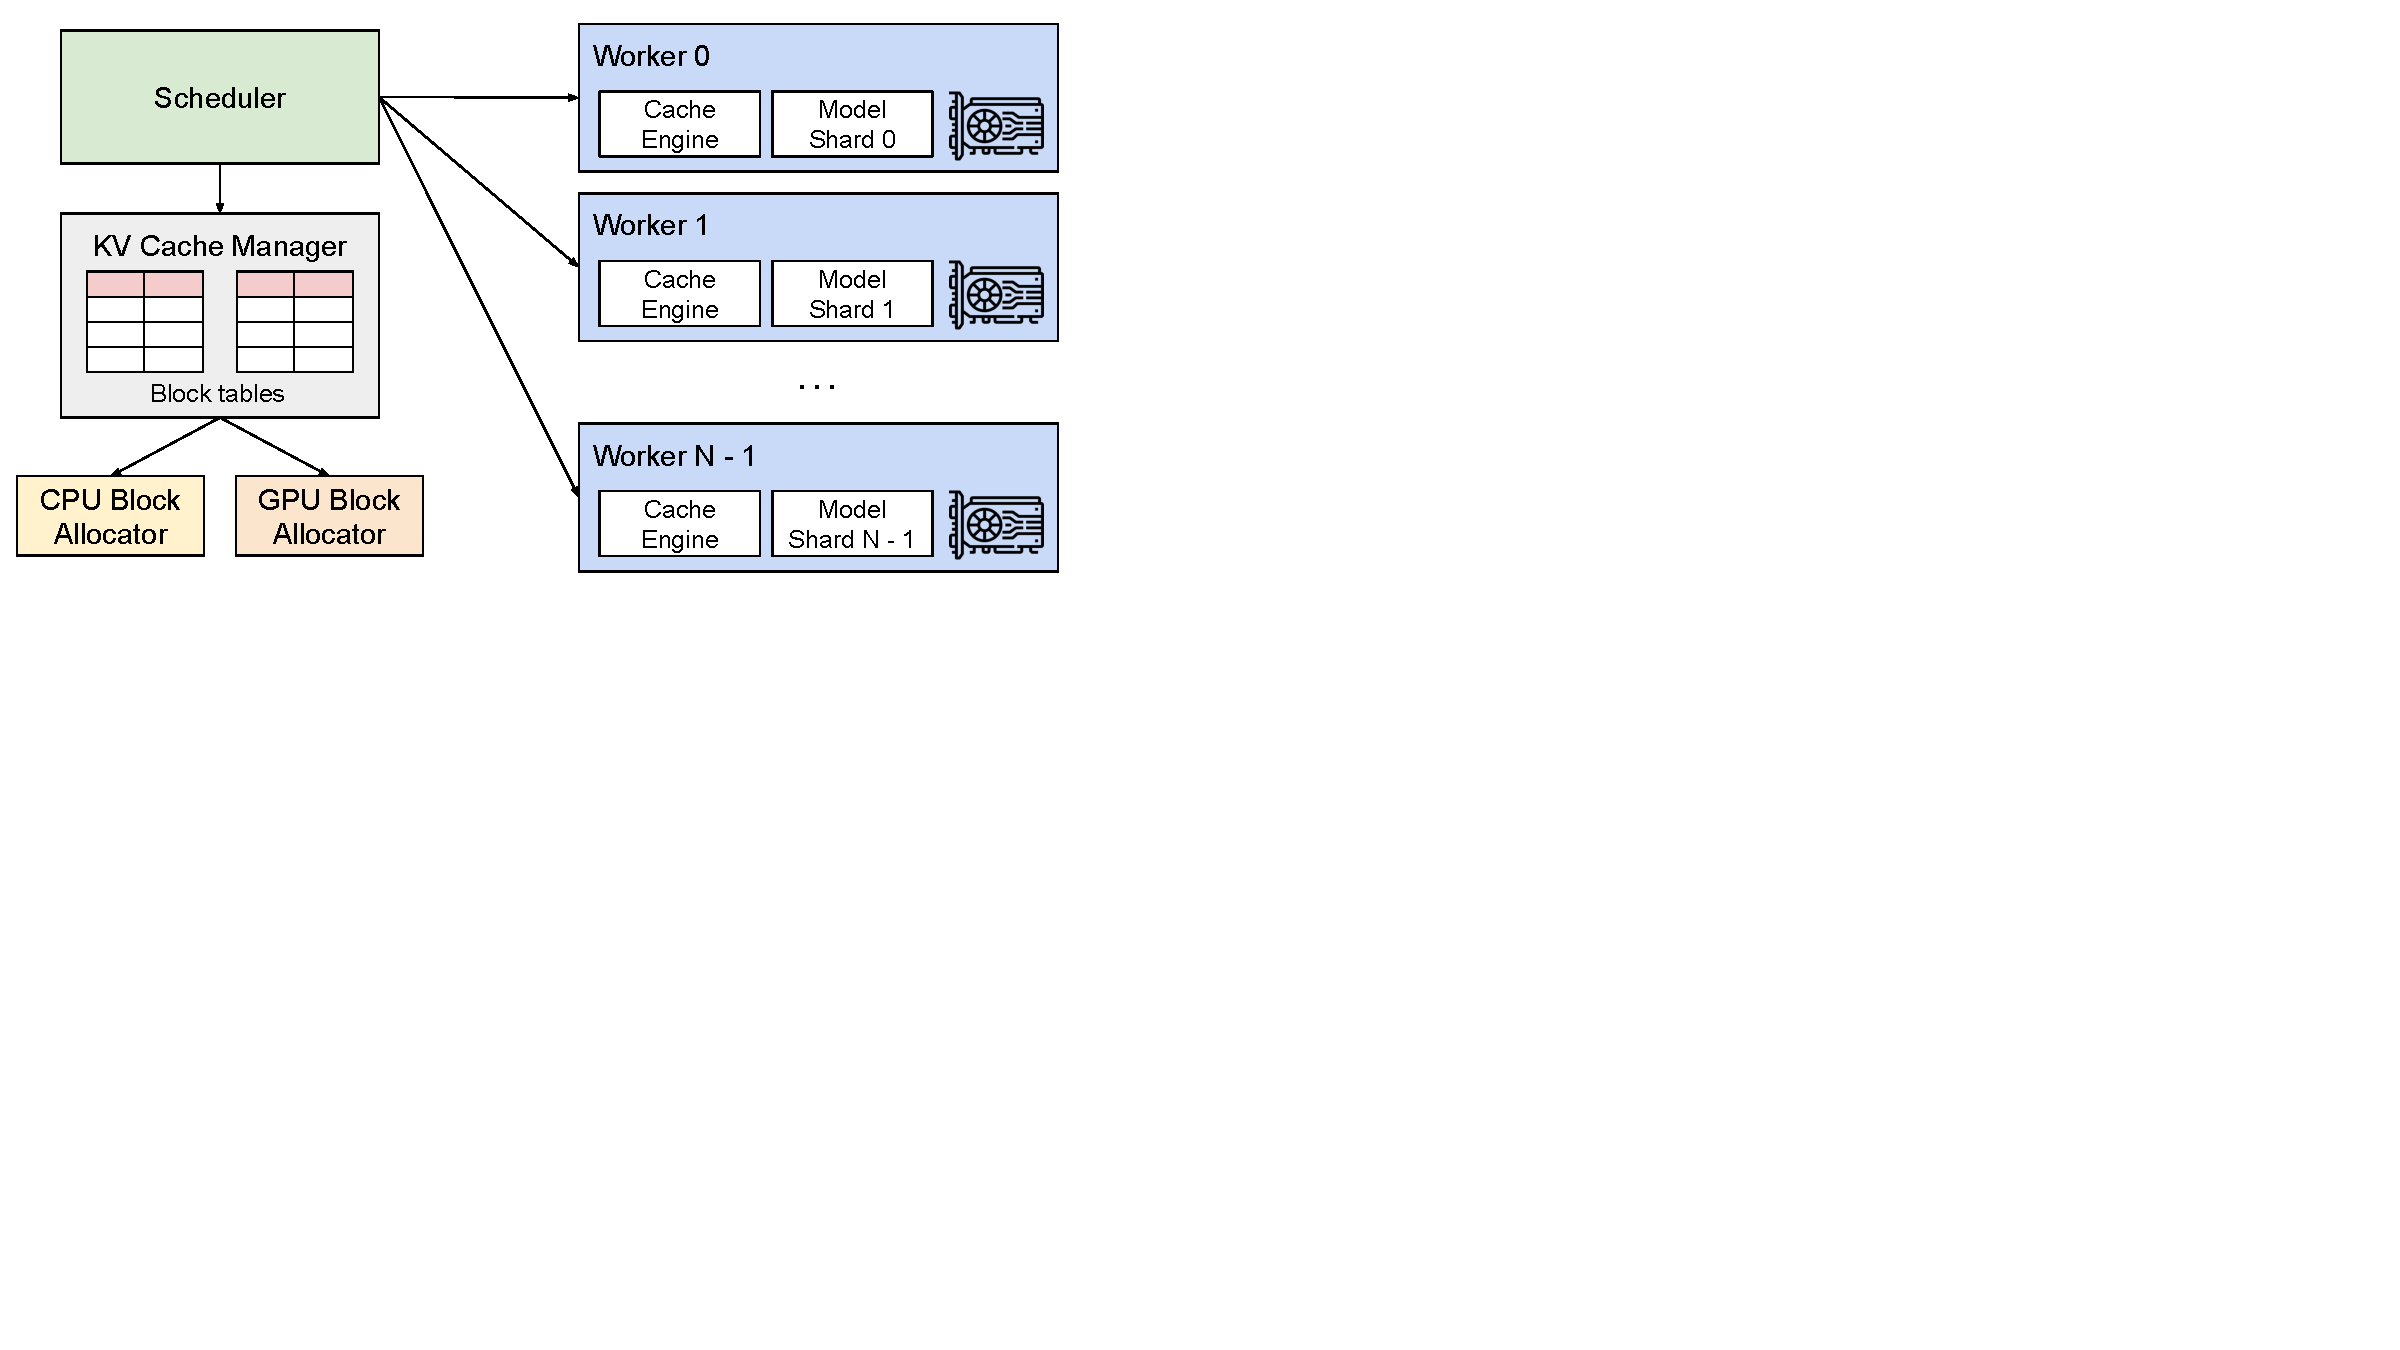
\includegraphics[width=\linewidth]{images/system-overview.pdf}
        \caption{System overview of vLLM.}
        \label{fig:vllm_overview}
    \end{subfigure}
    \hfill
    \begin{subfigure}[t]{0.54\linewidth}
        \centering
        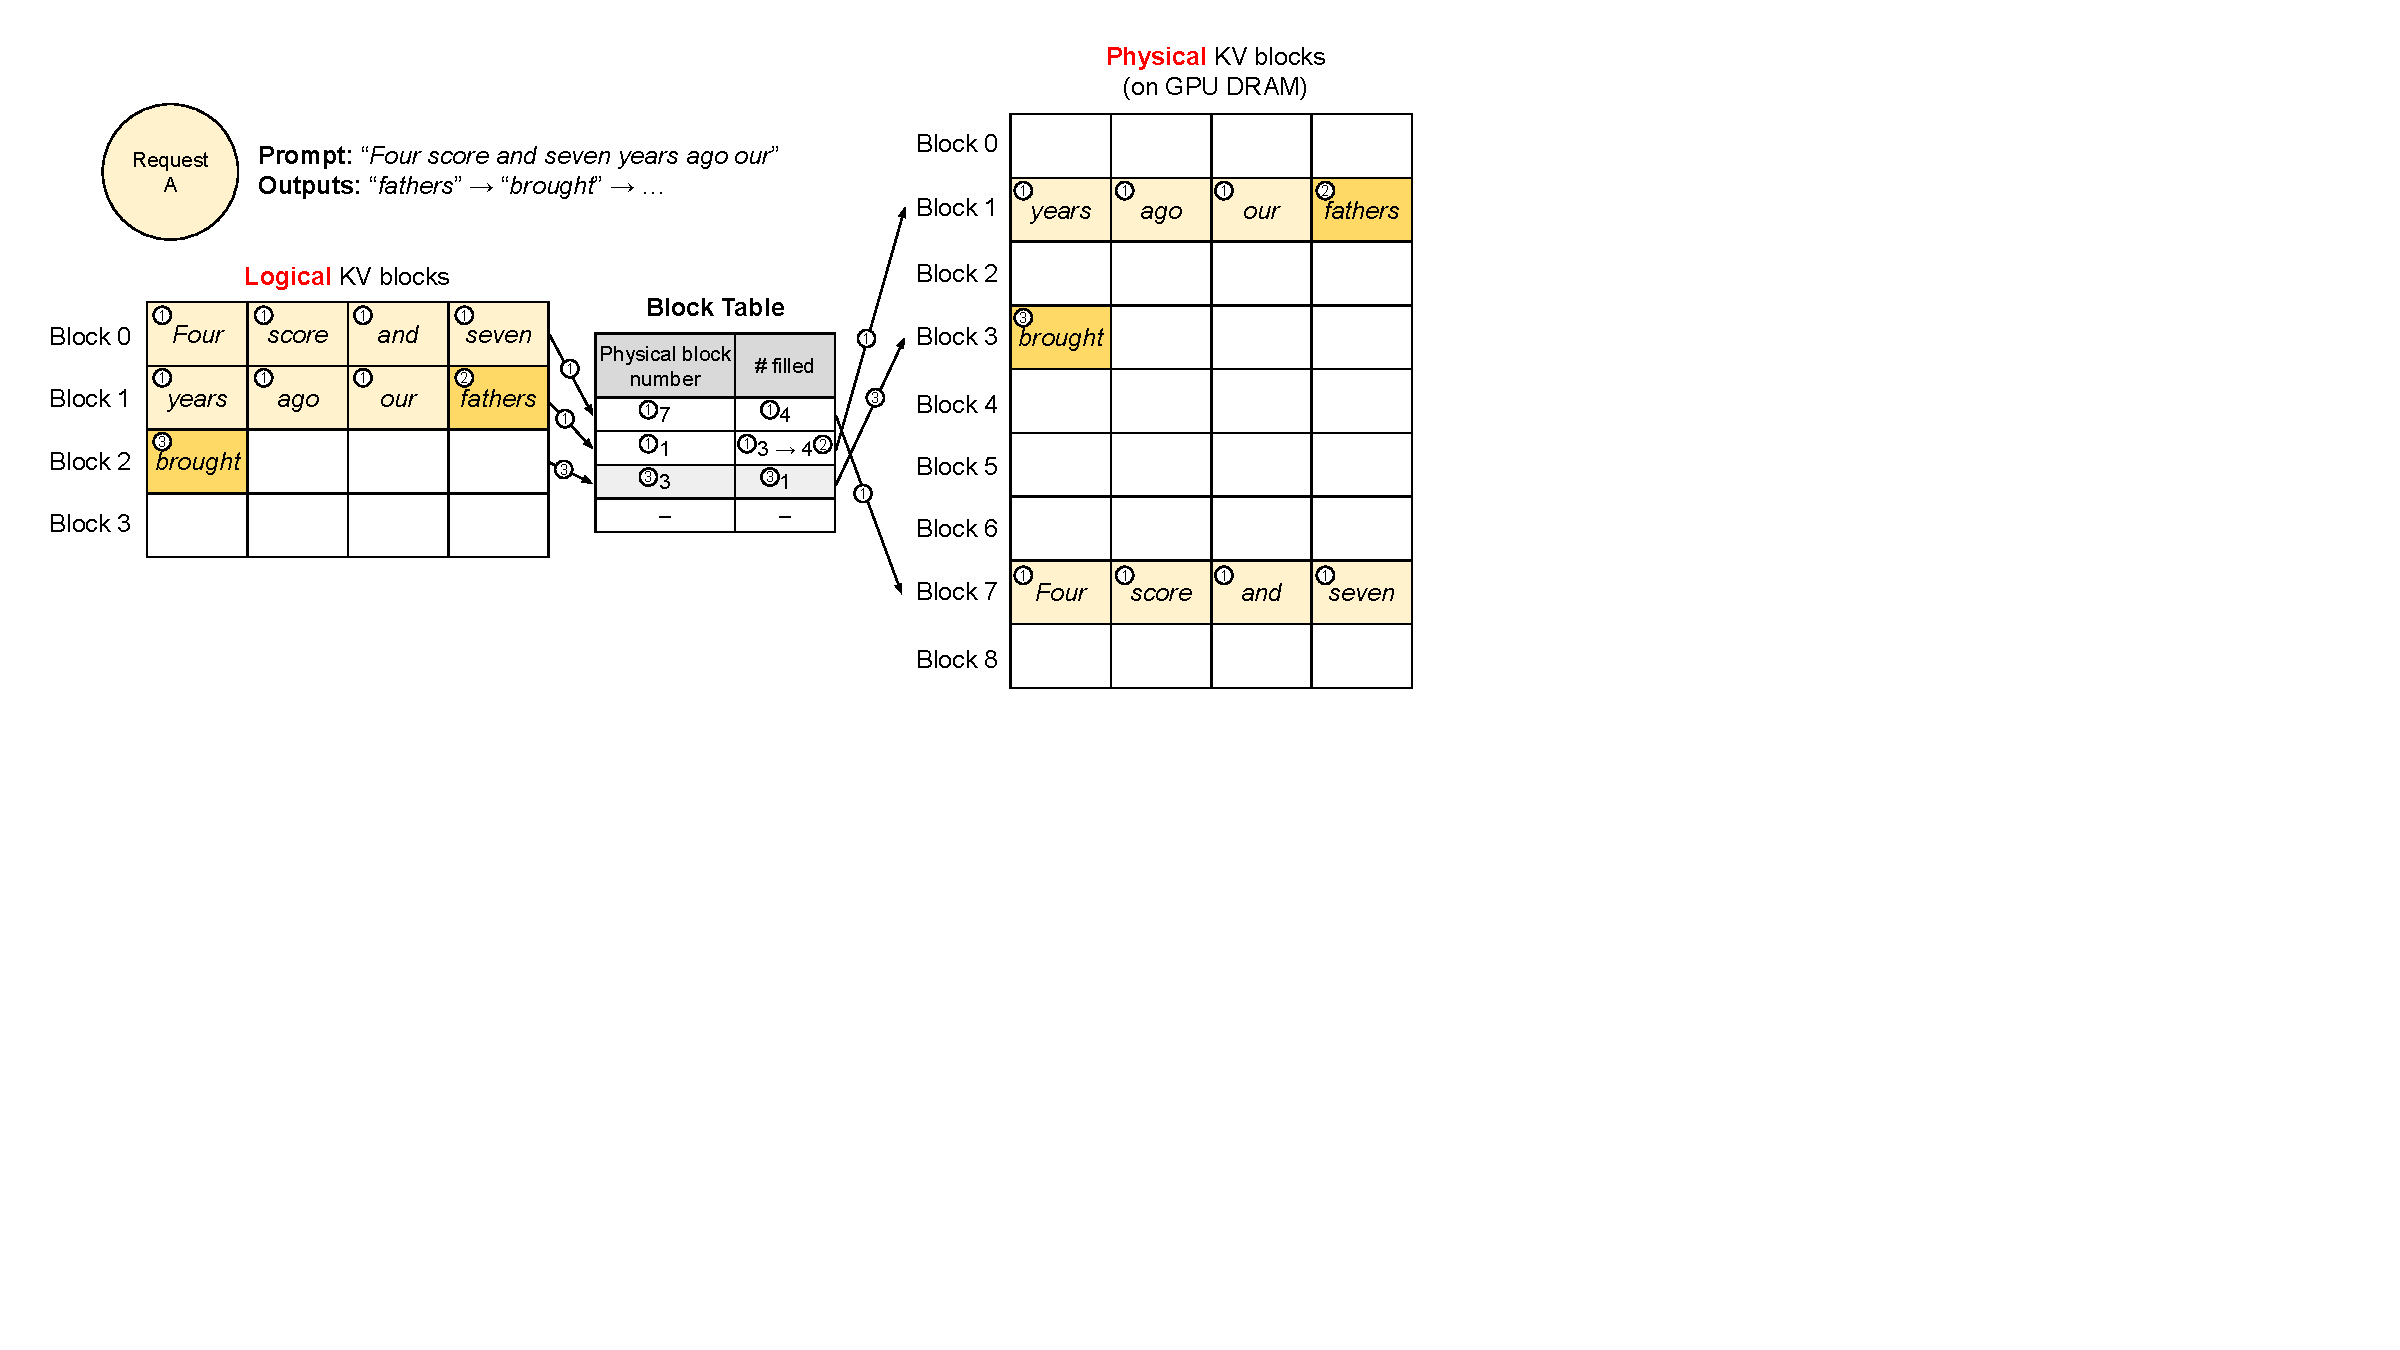
\includegraphics[width=\linewidth]{images/logical-and-physical-block-table.pdf}
        \caption{Block-based KV cache management in vLLM.}
        \label{fig:vllm_blocktable}
    \end{subfigure}
    \caption{Architecture and KV cache management in vLLM \cite{kwon2023vllm}.}
    \label{fig:vllm_case}
\end{figure}

Beyond memory allocation, vLLM also integrates dynamic scheduling to maintain high utilisation under heterogeneous workloads. Its scheduler can preempt requests when memory becomes tight, using either swapping or recomputation, and it works together with continuous batching to refill available capacity as requests complete. According to the vLLM paper, this integrated design improves throughput by 2--4$\times$ over prior serving systems at comparable latency \cite{kwon2023vllm}. From an operating-system perspective, vLLM is important because it combines paging, scheduling, and resource management into a unified system for efficient LLM inference.


\subsection{SGLang}

% Cover:
%   - RadixAttention: organises prefix blocks in a radix tree for O(L) lookup
%   - Automatic reuse without manual cache key specification
%   - Particularly effective for multi-turn conversations and agentic workflows
%   - Cite: Zheng et al. 2024

SGLang is a structured generation runtime that improves KV cache
efficiency by exploiting the structural regularity of real-world
workloads, such as shared system prompts, multi-turn dialogues,
and agentic pipelines \cite{zheng2024sglang}. Whereas vLLM focuses
primarily on block-level memory allocation, SGLang addresses a
complementary challenge: how to maximise cache reuse across requests
automatically, without requiring changes to application logic.

The central contribution of SGLang is \emph{RadixAttention}, which
organises KV cache blocks in a radix tree over token prefixes.
When a new request arrives, the runtime traverses the tree to find
the longest cached prefix and allocates memory only for the uncached
suffix. The tree is then maintained as execution proceeds so that
cached prefixes can be reused by later requests. Unlike vLLM's
hash-based prefix caching, this process is fully automatic and does
not require manual cache-key specification. Shared prefix blocks are
retained in a way that is analogous to copy-on-write sharing in Unix
processes, although the analogy is at the systems-design level rather
than a literal OS mechanism.

SGLang reports strong throughput gains on workloads with substantial
prefix overlap, such as multi-turn conversations and agentic
pipelines, but the benefit is workload-dependent and diminishes for
diverse one-shot queries \cite{zheng2024sglang}. In this sense,
SGLang complements the block-based allocation strategy of vLLM by
shifting the optimisation target from allocating cache pages
efficiently to maximising reuse across related requests.


\subsection{Side-by-Side Comparison}

Table~\ref{tab:system_compare} summarises the key differences between
vLLM and SGLang.
Despite sharing the same foundational primitives --- block-based KV cache
storage and continuous batching --- the two systems target distinct
bottlenecks in the serving pipeline.
vLLM prioritises efficient memory allocation and scheduling under pressure,
while SGLang prioritises automatic prefix reuse across structurally related
requests.

\begin{table}[htbp]
    \centering
    \caption{Comparison of KV cache management strategies in vLLM
    \cite{kwon2023vllm} and SGLang \cite{zheng2024sglang}.}
    \label{tab:system_compare}
    \begin{tabular}{p{3.8cm} p{4.6cm} p{4.6cm}}
        \toprule
        \textbf{Feature} & \textbf{vLLM}
                         & \textbf{SGLang} \\
        \midrule
        Primary goal
            & Reduce fragmentation and improve allocation efficiency
            & Maximise automatic KV cache reuse across requests \\
        Allocation unit
            & Fixed-size blocks (pages)
            & Fixed-size blocks (pages) \\
        Prefix caching
            & Hash-based, explicit prefix matching
            & Automatic radix-tree traversal (RadixAttention) \\
        Scheduling
            & Continuous batching
            & Continuous batching with cache-aware scheduling \\
        Preemption policy
            & Swap to CPU or recompute
            & Swap to CPU or recompute \\
        Best-suited workload
            & Heterogeneous high-throughput serving
            & Multi-turn, agentic, and prefix-overlapping workloads \\
        OS analogy
            & Virtual memory paging and page-table translation
            & Shared memory with copy-on-write semantics \\
        CPU swapping support
            & Full support
            & Partial support \\
        \bottomrule
    \end{tabular}
\end{table}

From an operating-systems perspective, the contrast between the two
systems is instructive.
vLLM addresses the classical problems of dynamic allocation, external
fragmentation, and preemptive scheduling under memory pressure ---
challenges that map directly onto virtual memory management
\cite{silberschatz2018os}.
SGLang, by contrast, emphasises sharing and reuse across related
execution contexts: requests with overlapping prefixes share the same
physical KV blocks until their paths diverge, at which point
copy-on-write semantics take effect \cite{zheng2024sglang}.
In this sense, vLLM exemplifies an OS-inspired \emph{allocation}
mechanism, while SGLang exemplifies an OS-inspired \emph{sharing}
mechanism.
Together, they demonstrate that KV cache management is not a single
optimisation trick, but a layered systems problem --- one that demands
solutions at the level of allocation, address translation, sharing, and
scheduling simultaneously.
% ============================================================
%  SECTION 6 — ANALYSIS  *** AT LEAST 1/5 of total — YOUR WORK ***
% ============================================================
\section{Analysis}
\label{sec:analysis}

This section presents an original analysis of KV cache memory
management from an operating-systems perspective. The main argument is
that KV cache management is not merely an implementation detail of LLM
inference, but a genuine memory-management problem involving
allocation, sharing, reclamation, and scheduling under resource
constraints. At the same time, the analogy to classical operating
systems is not exact. Some ideas transfer well, while others break down
because LLM inference has distinctive access patterns and workload
structures.

\subsection{How Deep Does the OS Analogy Go?}

Table~\ref{tab:os_analogy} summarises the main correspondences between
classical OS memory-management concepts and KV cache techniques in LLM
serving systems.\cite{silberschatz2018os,tanenbaum2015modern}

\begin{table}[htbp]
    \centering
    \caption{Mapping between OS memory management concepts and KV cache techniques.}
    \label{tab:os_analogy}
    \begin{tabular}{p{5.5cm} p{7cm}}
        \toprule
        \textbf{OS Concept} & \textbf{KV Cache Equivalent} \\
        \midrule
        Virtual memory paging         & PagedAttention block table \\
        Page table / TLB              & Block table lookup in vLLM \\
        Copy-on-write (CoW fork)      & Shared prefix blocks with CoW \\
        Swapping to disk              & KV offloading to CPU / NVMe \\
        Preemptive process scheduling & Continuous batching + preemption \\
        Shared memory segments        & Cross-request shared prefix blocks \\
        Demand paging                 & Not yet implemented; open challenge \\
        \bottomrule
    \end{tabular}
\end{table}

The analogy is strongest at the level of mechanisms. Paging and
PagedAttention are closely related because both use fixed-size blocks
and an indirection table to map logical positions to physical memory.
Swapping also has a clear parallel: KV offloading moves cached states
from fast GPU memory to slower storage when capacity becomes tight.
Similarly, prefix sharing resembles copy-on-write, since multiple
requests can reuse the same cached prefix until their execution paths
diverge.

However, the analogy weakens when one considers execution semantics.
Classical demand paging is lazy, whereas KV cache states are usually
written eagerly during prefill. In addition, OS memory access is
general and potentially random, while KV cache access during decoding is
highly structured and largely sequential. This makes KV cache
management more predictable in some respects, even though eviction and
scheduling remain difficult.

Another important difference is isolation. Operating systems provide
each process with a protected address space, whereas LLM serving systems
typically manage many requests within one shared KV cache pool. Prefix
sharing can therefore improve efficiency, but it also creates a
potential isolation problem if blocks are not carefully protected. For
this reason, the OS analogy is best understood as a mechanism-level
framework rather than a literal one-to-one mapping.


\subsection{Trade-off Analysis: Block Size Selection in PagedAttention}

A natural question arising from the PagedAttention design is how to
choose the block size $B$ --- the number of tokens stored in each
fixed-size KV cache block.
Although vLLM defaults to $B = 16$, this choice is not arbitrary, and
understanding the trade-off it encodes reveals a deeper connection to
classical OS page-size selection problems.

\paragraph{A simple fragmentation model.}
For a sequence of length $s$ tokens, the number of blocks required is
$\lceil s / B \rceil$.
The last block is, on average, half-full, so the expected internal
fragmentation per sequence is approximately $B/2$ tokens.
Expressed as a fraction of the total sequence length, the fragmentation
ratio is:
\begin{equation}
    f(s, B) = \frac{B/2}{s} = \frac{B}{2s}
    \label{eq:frag}
\end{equation}
This shows that fragmentation is proportional to $B$ and inversely
proportional to $s$: large blocks hurt short sequences disproportionately.
For example, with $B = 16$ and a short sequence of $s = 32$ tokens,
up to 25\% of allocated memory may be wasted on average.
For a longer sequence of $s = 1024$ tokens, the same block size wastes
less than 1\%.

\paragraph{The cost of small blocks.}
Reducing $B$ lowers fragmentation but introduces two counteracting costs.
First, the block table grows: each sequence requires
$\lceil s / B \rceil$ entries, so halving $B$ doubles the number of
table lookups and pointer-chasing operations during attention computation.
Second, smaller blocks reduce memory access locality.
Modern GPU memory systems perform best when consecutive memory accesses
fall within the same contiguous region; splitting a sequence across many
small non-contiguous blocks increases the number of distinct memory
transactions required per attention step, reducing effective memory
bandwidth utilisation.

\paragraph{The cost of large blocks.}
Conversely, increasing $B$ reduces table overhead and improves access
locality, but fragmentation grows linearly with $B$ according to
Equation~\ref{eq:frag}.
For workloads dominated by short sequences --- such as classification or
single-turn queries --- a large block size can waste a substantial
fraction of GPU memory, directly reducing the maximum batch size and
therefore throughput.
Furthermore, large blocks make memory preemption coarser: when the
scheduler must evict a partially used block to free memory, the entire
block must be swapped or recomputed, even if only a few of its token
slots are occupied.

\paragraph{Evaluating vLLM's default choice.}
vLLM selects $B = 16$ as its default \cite{kwon2023vllm}.
Substituting into Equation~\ref{eq:frag}, this wastes at most 8 tokens
per sequence, which is negligible for the typical serving workload of
hundreds to thousands of tokens per request.
At the same time, a block table of depth $\lceil s/16 \rceil$ remains
small enough that lookup overhead is not a bottleneck.
This choice mirrors the reasoning behind OS page-size selection, where
4\,KB pages represent a similar compromise between fragmentation and
table overhead for general-purpose workloads \cite{silberschatz2018os}.

However, the analogy also exposes a limitation.
OS kernels support \emph{huge pages} (2\,MB or 1\,GB) for workloads
with large, contiguous memory footprints, reducing TLB pressure at the
cost of higher fragmentation.
An analogous mechanism for KV cache --- dynamically adjusting block
size based on observed sequence length distribution --- does not yet
exist in production systems.
For very long contexts ($s \geq 100\,000$ tokens), the block table itself
becomes non-trivial in size, and a larger $B$ would be preferable.
For short-sequence workloads, a smaller $B$ would reduce waste.
This suggests that a \emph{workload-adaptive block size}, similar in
spirit to transparent huge pages in Linux, is a promising direction for
future work.
\subsection{When Does Prefix Caching Help?}

Prefix caching is sometimes presented as a universal win, but its
benefit depends critically on the structure of the incoming workload.
Two factors jointly determine the practical gain: the \emph{prefix
hit rate} $h$ (the fraction of requests that share a cached prefix)
and the \emph{prefix coverage ratio} $r = l_p / s$ (the proportion of
the total sequence length accounted for by the shared prefix, where
$l_p$ is the prefix length and $s$ is the full sequence length).
The expected saving in prefill computation is proportional to $h \cdot r$;
when either factor is small, the benefit is marginal.

Table~\ref{tab:prefix_workload} analyses three representative workload
types under this framework.

\begin{table}[htbp]
    \centering
    \caption{Prefix caching effectiveness across workload types.}
    \label{tab:prefix_workload}
    \begin{tabular}{p{3.2cm} p{2.4cm} p{2.4cm} p{2.4cm} p{2.4cm}}
        \toprule
        \textbf{Workload} & \textbf{Hit rate $h$}
        & \textbf{Coverage $r$} & \textbf{Net gain}
        & \textbf{Recommendation} \\
        \midrule
        Chatbot with fixed system prompt
            & High ($\approx$1.0) & Medium (0.2--0.5)
            & High & Always enable \\
        One-shot diverse queries
            & Near zero & Near zero
            & Negligible & Overhead not justified \\
        Batch document processing (shared template)
            & Medium (0.5--0.8) & Low (0.1--0.2)
            & Moderate & Enable with profiling \\
        \bottomrule
    \end{tabular}
\end{table}

Prefix caching also carries overhead that is absent in plain paged
allocation: the runtime must maintain a hash table or radix tree,
retain completed requests' blocks in memory speculatively, and perform
cache-aware scheduling to avoid thrashing \cite{zheng2024sglang}.
For workloads with low hit rates, these costs are pure waste.
This analysis suggests that prefix caching should be treated as a
workload-specific optimisation rather than a default-on feature:
operators should profile their traffic to estimate $h$ and $r$ before
enabling it in production.

% ============================================================

\subsection{Limitations and Open Challenges}

Despite the progress surveyed in previous sections, several important
problems remain unsolved.

\paragraph{Distributed KV cache management.}
Large models are typically served with tensor parallelism, which
partitions attention heads across multiple GPUs.
This means the KV cache for a single request is inherently distributed,
and the block table abstraction used by vLLM becomes per-GPU rather
than global \cite{kwon2023vllm}.
Cross-node prefix sharing would require network communication whose
latency is orders of magnitude higher than a local block-table lookup,
making the radix-tree approach of SGLang difficult to extend to
multi-node deployments \cite{zheng2024sglang}.
A coherent, distributed KV cache management layer analogous to a
distributed shared-memory system remains an open problem.

\paragraph{Very long contexts.}
Applying Equation~\ref{eq:kvcost} to a 1M-token sequence on a 70B
model yields a KV cache footprint exceeding 100\,GB --- far beyond the
HBM capacity of any current GPU.
Hierarchical offloading to CPU DRAM and NVMe, as demonstrated by
FlexGen \cite{sheng2023flexgen}, can extend the effective memory
capacity, but the bandwidth gap between GPU HBM ($\sim$2\,TB/s), PCIe
($\sim$32\,GB/s), and NVMe ($\sim$7\,GB/s) imposes severe latency
penalties.
Closing this gap without sacrificing interactive latency is an
unsolved engineering challenge.

\paragraph{Multimodal KV caches.}
Vision encoders such as ViT typically produce 256--1024 tokens per
image, and the number varies with resolution.
This variability breaks the fixed-block-size assumption of PagedAttention
and complicates eviction policies designed for text: vision tokens
relevant to the current query may need to be retained throughout the
conversation, while text tokens from earlier turns may safely be evicted.
Existing policies such as H2O \cite{zhang2023h2o} and StreamingLLM
\cite{xiao2024streamingllm} do not account for this modality-specific
importance distinction, leaving multimodal KV cache management largely
unaddressed.

\paragraph{Privacy and isolation.}
Shared prefix blocks allow different users' requests to occupy the same
physical GPU memory, which introduces a risk absent in OS-managed
processes: without explicit isolation guarantees, a side-channel attack
could potentially infer the content of another user's KV blocks ---
including proprietary system prompts or conversation history.
Operating systems address analogous risks through address space
isolation and memory protection hardware \cite{silberschatz2018os},
but current LLM serving systems provide no equivalent mechanism.
As inference services become more widely deployed, this gap between
OS-level security principles and LLM runtime practice warrants serious
attention.
% ============================================================
%  SECTION 7 — CONCLUSION
% ============================================================
\section{Conclusion}
\label{sec:conclusion}

KV cache management has become a central systems problem in modern LLM
inference, because serving performance is increasingly limited not only
by computation but also by memory capacity, allocation efficiency, and
data movement. As this report has shown, many of the key techniques
used in current inference systems --- including PagedAttention, prefix
sharing, continuous batching, and KV offloading --- can be understood
through the lens of classical operating-system memory management
\cite{kwon2023vllm,zheng2024sglang}. This OS perspective is useful not
only as an analogy, but also as a practical framework for reasoning
about fragmentation, sharing, preemption, and resource utilisation in
real serving systems.

At the same time, the analysis in this report shows that the analogy is
not exact. KV cache management differs from traditional OS memory
management in its sequential access pattern, eager prefill behaviour,
and weaker isolation across requests. These differences mean that
classical ideas such as paging and copy-on-write remain highly
valuable, but they must be adapted to the specific constraints of LLM
workloads rather than applied mechanically.

Overall, systems such as vLLM and SGLang demonstrate that OS-inspired
design can translate into substantial practical gains in throughput and
memory efficiency. However, important challenges remain, especially for
distributed serving, extremely long contexts, multimodal workloads, and
privacy-preserving cache sharing. Future progress will likely depend on
continued cross-fertilisation between operating-systems research and
LLM inference systems, with KV cache management remaining a key area of
innovation.



% ============================================================
%  REFERENCES
% ============================================================
\newpage
\bibliographystyle{IEEEtran}
\bibliography{references}

\end{document}